\documentclass[a4paper, 12pt]{article}
\usepackage[utf8]{inputenc}
\usepackage[english,swedish]{babel}
\usepackage{cite}
%\usepackage[backend=bibtex]{biblatex}
%\addbibresource{kallor.bib}
%\usepackage{times}

\usepackage{tikz}
\usetikzlibrary{shadows}
\newcommand*\key[1]{%
  \tikz[baseline=(key.base)]
    \node[%
      draw,
      fill=white,
      drop shadow={shadow xshift=0.25ex,shadow yshift=-0.25ex,fill=black,opacity=0.75},
      rectangle,
      rounded corners=2pt,
      inner sep=1pt,
      line width=0.5pt,
      font=\scriptsize\sffamily
    ](key) {#1\strut}
  ;
}

\title{Kassa\\\large en enkel kassa mjukvara}
\author{Sam Sadeghi SY17}
\date{2019/2020}

 
\begin{document}
\begin{titlepage}
\maketitle
\end{titlepage}

\selectlanguage{english}

\begin{abstract}

\end{abstract}
\selectlanguage{swedish}
\newpage
\tableofcontents
\newpage

\section{Inledning}
Ibland hjälper jag min farbror i hans livsmedel butik. 
Där får jag använd använda mig av kassaapparaten. 
Programmet som kassaapparaten på farbrors butik kör är långsamt och jag tänkte att jag skulle kunna göra ett liknande program som kör snabbare genom att endast ha med de nödvändigaste funktionerna.

\subsection{Syfte}

I skapandet av det här programmet ska jag lära mig hur man gör ett grafisk program med hjälp av programmerings språket Python och gränssnitsverktyget Tkinter. 

\subsection{Mål}

Vid slutet av arbetet ska jag ha ett enkelt kassa program som kan räkna ihop summan av flera varor samt hur mycket moms som skall betala beroende på varans typ. Programmet skall även kunna skriva ut ett kvitto 

\subsection{Metod}

Redskap jag kommer använda är


Vim:\\
Vim är ett text redigerings program som körs i konsolen.
Det finns massor med fördelar med Vim.
En av dessa fördelar är att den inte tar lika mycket resurser att köra Vim som till exempel Visual Studio men det i sig är inte så viktigt utan den största anledningen till varför jag jag använde Vim för att skriva det här programmet är att jag har vant mig vid Vims massor med tangentbords-genvägar och det hjälper mig skriva snabbare inte bara det utan jag är också väldigt bekväm med att konfigurera Vim så att lättare kan skriva.
Ett av dessa konfigurationer jag har gjort för att underlätta mitt skapande av programmet är att jag har gjort så att när jag trycker ner på \key{Ctrl } och \key{W} samtidigt så startar den programmet. Andra program kan säkert görande någonting liknade eller kanske till och med kommer inbyggt med en sådan funktion men i Vim får jag göra det det själv som får mig att bättre förstå vad som händer i bakgrunden och som sagt tidigare är jag mycket bekvämare med Vim än vad jag är med andra text redigerings program


Python:\\
% läs mer om TIOBE
% läs https://medium.com/@mindfiresolutions.usa/python-7-important-reasons-why-you-should-use-python-5801a98a0d0b
Python är ett programmeringsspråk.
Jag valde just Python för att skriva det här programmet för att jag ser det väldigt ofta i min omgivning.
Enligt TIOBE indexet \cite{TIOBE} är Python det tredje populäraste språket och dess popularitet värkar öka (se figur \ref{fig:index_python}) till skillnad från språket som ligger på första plats det vill säga Java (se figur \ref{fig:index_java}) och ju populärare ett programmeringsspråk är så finns det fler projekt som är skrivna i de programmeringsspråket därför tycker jag att det är värt att lära sig /skriva i  Python.


\begin{figure}[h!]
  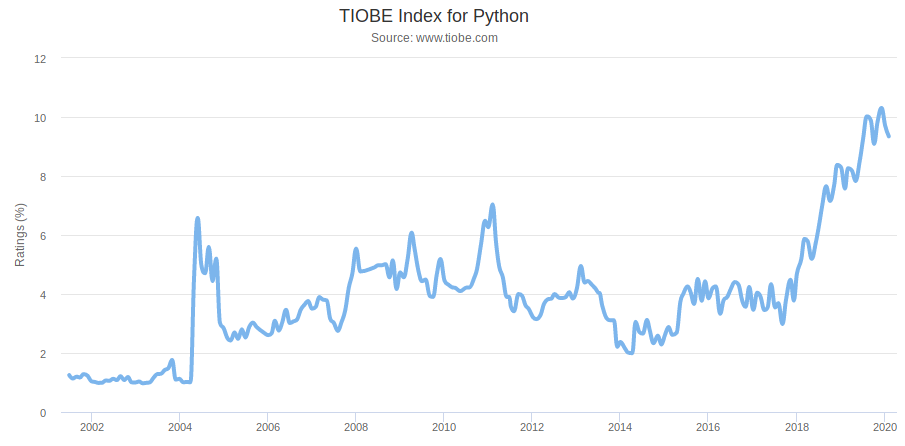
\includegraphics[width=\linewidth]{img/TIOBE_python.png}
  \caption{TIOBE index för python}
  \label{fig:index_python}
\end{figure}
\begin{figure}[h!]
  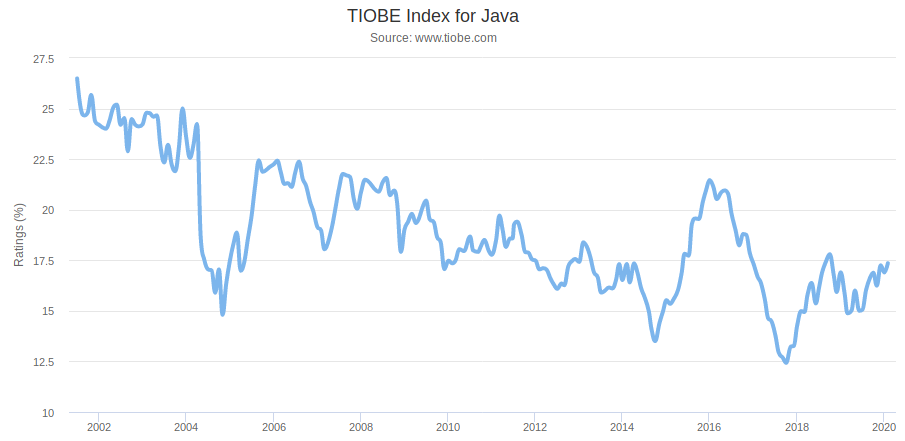
\includegraphics[width=\linewidth]{img/TIOBE_java.png}
  \caption{TIOBE index för java}
  \label{fig:index_java}
\end{figure}


Tkinter/TK:\\
Tkinter är en API för att använda TK i Python. 
TK är grafiskt gränssnits verktyg som fungerar på Windows, MacOS och Linux. 
Jag valde Tkinter på grund av att den fungerar på dom tre vanligare operativsystemen.
Tkinter kommer 


FPDF:\\
FPDF är ett programbibliotek för att generera PDF filer.
PDF filer är dokument filer som är optimerade för att skrivas ut.


Github och Git:\\
Github är en webbserver med fokus på program utveckling. 
Github använder sig av version kontroll programmet Git. 
Git gör det enkelt för mig att se vad jag har gjort och när jag har gjort det.
Git tillsammans med Github låter mig jobba på programmet var jag än är utan att vara uppkopplad till internet.

\section{Utförande}

\section{Resultat}

\section{Diskussion}

\section{Slutsats}

\newpage 

\bibliography{main}{}
\bibliographystyle{ieeetr}

%\printbibliography

\end{document}
